\section{Auswertung}
\label{sec:Auswertung}

Die Materialeigenschaften der auf der Grundplatte verbauten Stäbe werden der Versuchsdurchführung entnommen und in Tabelle \ref{tab:1} angegeben.

\begin{table}
  \centering
  \caption{Materialeigenschaften der Grundplatte. \cite{sample}}
  \label{tab:1}
  \sisetup{table-format=1.2}
  \begin{tabular}{c c c c c c}
    \toprule
    {$\text{Material}$} & {$l \:/\: \si{\centi\metre}$} & {$b \:/\: \si{\centi\metre}$} & {$h \:/\: \si{\centi\metre}$} & {$\rho \:/\: \si{\kilo\gram\per\metre\tothe{3}}$} & {$c \:/\: \si{\joule\per\kilo\gram\per\kelvin} $} \\
    \midrule
    Messing  & 9 & 1.2 & 0.4 & 8520 & 385 \\
    Messing  & 9 & 0.9 & 0.4 & 8520 & 385 \\
    Aluminium  & 9 & 1.2 & 0.4 & 2800 & 830 \\
    Edelstahl  & 9 & 1.2 & 0.4 & 8000 & 400 \\

    \bottomrule
  \end{tabular}
\end{table}

Zunächst wird die erste Messung, wie in Kapitel \ref{sec:stat} beschrieben, durchgeführt.


\subsection{Qualitative Beschreibung des Temperaturverlaufes}


In Abbildung \ref{fig:1} wird der zeitliche Verlauf für $T_1$ und $T_4$ dargestellt, in \ref{fig:2} der zeitliche Verlauf von $T_5$ und $T_8$.

\begin{figure}
  \centering
  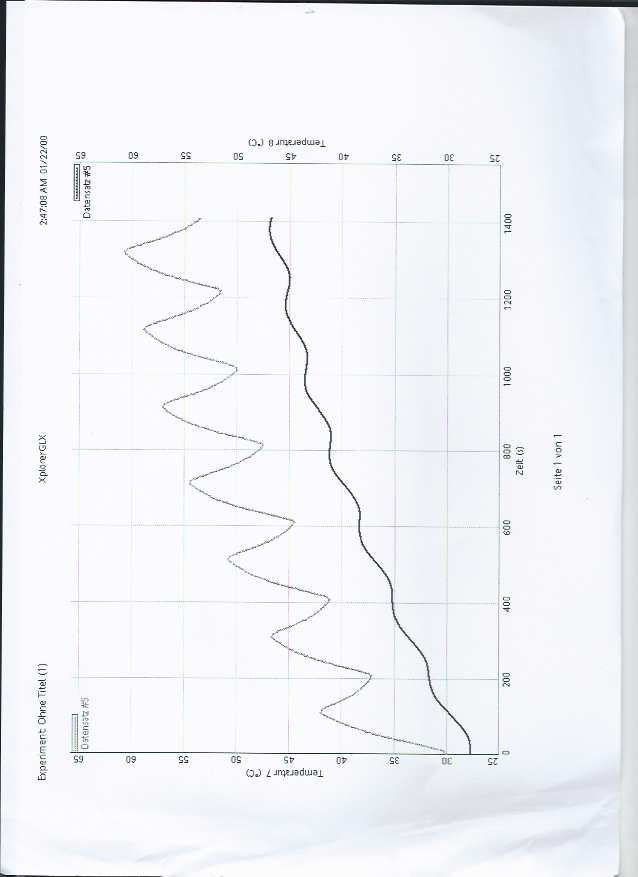
\includegraphics[height=13cm, angle=270]{scan-7.jpg}
  \caption{Zeitlicher Temperaturverlauf von $T_1$ und $T_4$.}
  \label{fig:1}
\end{figure}

\begin{figure}
  \centering
  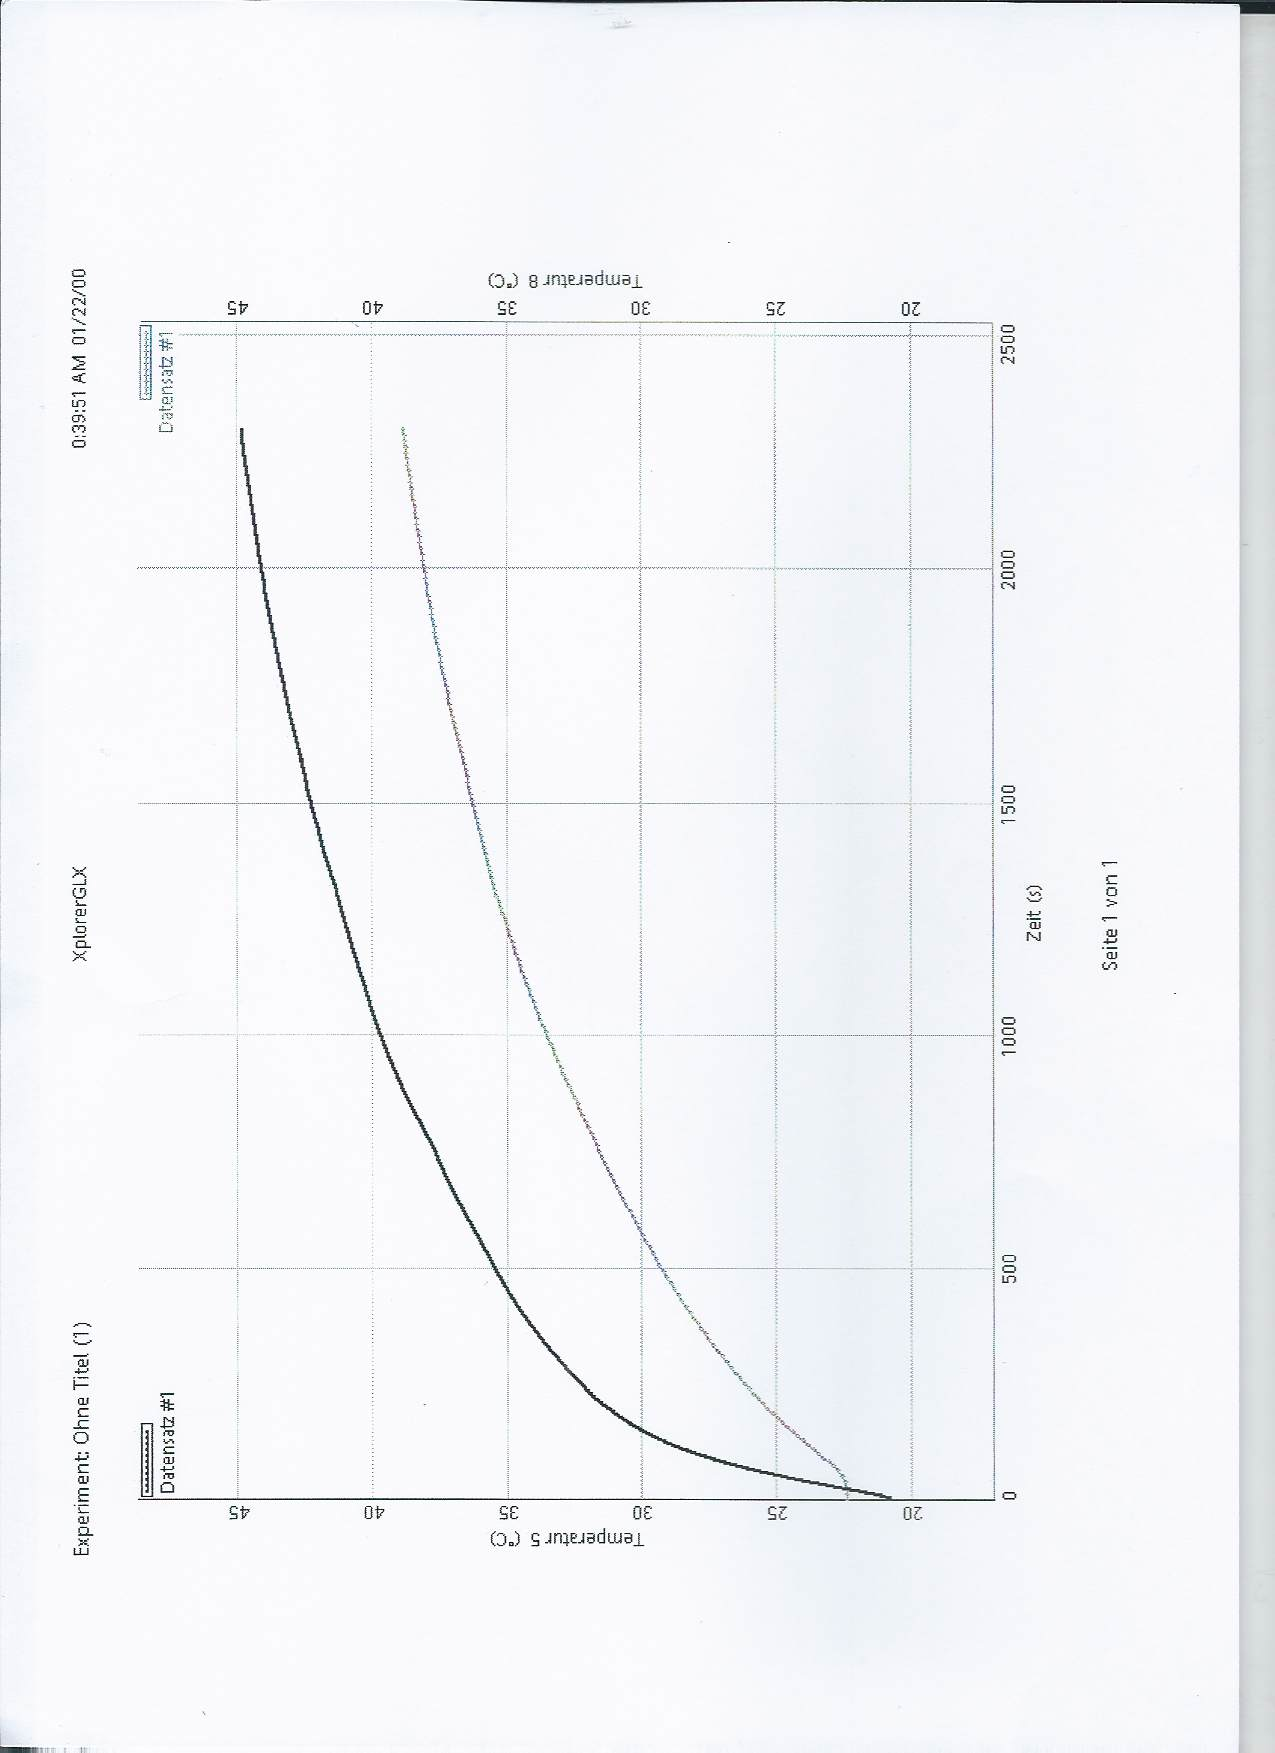
\includegraphics[height=13cm, angle=270]{scan-6.jpg}
  \caption{Zeitlicher Temperaturverlauf von $T_5$ und $T_8$.}
  \label{fig:2}
\end{figure}

Für Abbildung \ref{fig:1} fällt auf, dass beide Graphen eine ähnliche Form aufweisen.
Nach erst ca. $\SI{200}{\second}$ bildet sich eine Temperaturdifferenz, die nach ungefähr $\SI{500}{\second}$ konstant $\SI{1}{\kelvin}$ beträgt.
Die Graphen wachsen bis zum Ende der Messung in einer identischen Form weiter.
Diese Ähnlichkeiten lassen sich darauf zurückführen, dass es sich um das gleiche Material, nämlich Messing handelt.
Die Unterschiede werden durch die verschiedenen Ausmaße verursacht.\\
Für Abbildung \ref{fig:2} fällt auf, dass der Graph von $T_5$ eine zu Beginn stärkere Steigung aufweist als der Graph von $T_8$.
Nach einiger Zeit stellt sich eine annähernd konstante Temperaturdifferenz von ca. $\SI{6}{\kelvin}$ ein, welche bis zum Ende der Messung besetehen bleibt.
Grund hierfür ist, dass es sich beim ersten Material um Aluminium handelt, welches scheinbar eine bessere Wärmeleitfähigkeit als das andere Material, nämlich Edelstahl, besitzt.\\
Betrachtet man genauer die Temperaturen, welche für die verschiedenen Messpunkte nach $\SI{700}{\second}$ auftreten, so erhält man
\begin{align*}
  T_1 &= \SI{35.70}{\celsius}  \:\: \text{(Messing)}, \\
  T_4 &= \SI{34.73}{\celsius} \:\: \text{(Messing)}, \\
  T_5 &= \SI{37.26}{\celsius} \:\: \text{(Aluminium)}, \\
  T_8 &= \SI{31.14}{\celsius} \:\: \text{(Edelstahl}).
\end{align*}
Diese Werte führen zu der Annahme, dass die beste Wärmeleitfähigkeit bei Aluminium vorliegt, gefolgt von Messing, wobei hier die Wärmeleitfähigkeit von den Maßen abhängt.
Die geringste Wärmeleitfähigkeit kann dem Edelstahl zugeordnet werden.\\


\subsection{Bestimmung des Wärmestroms}


Der Wärmestrom, der zu einem bestimmten Zeitpunkt fließt, kann nach Gleichung \ref{eqn:w} berechnet werden.
Es werden dafür die Temperaturen $T_1$ und $T_2$, also von Messing betrachtet.
Die Temperaturdifferenzen können der Abbildung \ref{fig:3} entnommen werden, die weiteren Größen sind
\begin{align*}
  \increment{x} &= \input{build/x_ws.tex}\si{\metre} \\
  A &= \input{build/a_ws.tex}\si{\metre\tothe{3}} \\
  \kappa_\text{Messing} &= \input{build/k_ws.tex}\si{\watt\per\metre\per\kelvin} \\
\end{align*}
wobei $\increment{x}$, der Abstand der Messstellen, am Aufbau abgelesen wird, der Querschnitt $A$ aus Tabelle \ref{tab:1} errechnet und $\kappa_\text{Messing}$ der Literatur entnommen wird.
Es ergeben sich somit die in Tabelle \ref{tab:2} angegebenen Wärmeströme für die jeweligen Messzeiten.

\begin{table}
  \centering
  \caption{Wärmeströme für Messing.}
  \label{tab:2}
  \sisetup{table-format=1.2}
  \begin{tabular}{c c}
    \toprule
    {$t \:/\: \si{\second}$} & {$\frac{\increment{Q}}{\increment{t}} \:/\: \si{\watt}$}\\
    \midrule
    \input{build/wstrom.tex}
    \bottomrule
  \end{tabular}
\end{table}

Zuletzt werden die Temperaturdifferenzen zwischen dem Ende sowie dem Anfang des Stabes gegen die Zeit abgetragen.
Es ergibt sich für Messing der in Abbildung \ref{fig:3} dargestellte Graph, für Edelstahl der in Abbildung \ref{fig:4} dargestellte Graph.
\begin{figure}
  \centering
  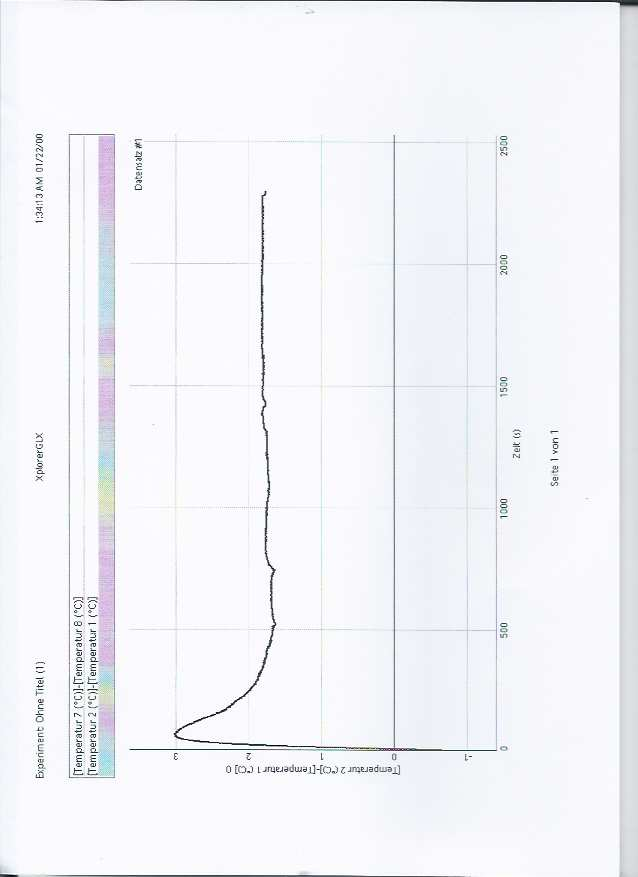
\includegraphics[height=13cm, angle=270]{scan-4.jpg}
  \caption{Zeitlicher Verlauf der Temperaturdifferenz von $T_2$ zu $T_1$.}
  \label{fig:3}
\end{figure}

\begin{figure}
  \centering
  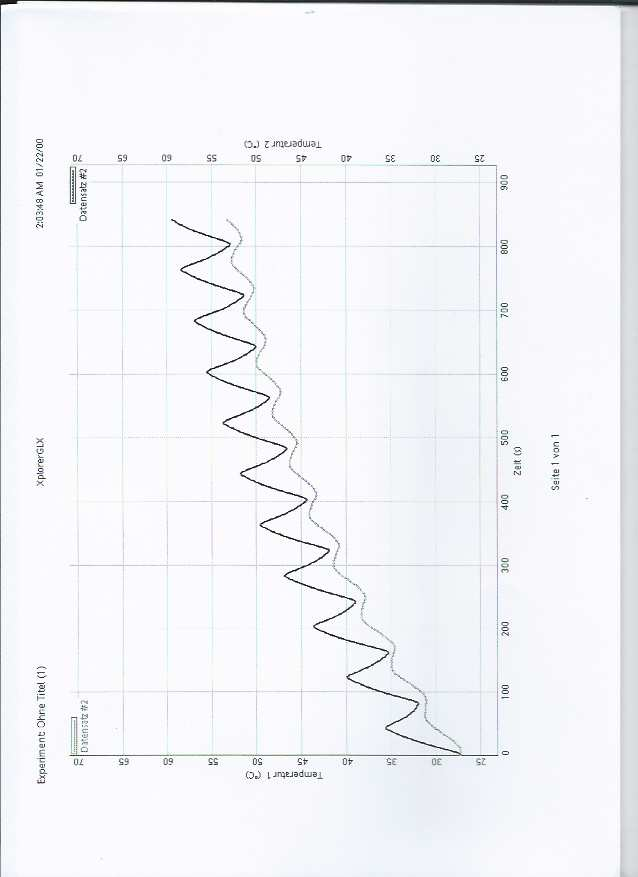
\includegraphics[height=13cm, angle=270]{scan-5.jpg}
  \caption{Zeitlicher Verlauf der Temperaturdifferenz von $T_7$ zu $T_8$.}
  \label{fig:4}
\end{figure}

Beide Graphen zeigen zu Beginn eine Temperaturdifferenz von $\SI{0}{\kelvin}$ auf, welche innerhalb der nächsten ca. $\SI{100}{\second}$ bis auf $\SI{6.5}{\kelvin}$ für Edelstahl bzw. $\SI{3}{\kelvin}$ Kelvin für Messing ansteigt.
Beim Messing ist hier ein starker Peak zu betrachten, im weiteren Verlauf sinkt die Temperaturdifferenz wieder auf ein bis zum Ende der Messung konstantes Nievau von ca. $\SI{1.7}{\kelvin}$ ab.
Im Gegensatz dazu befindet sich beim Edelstahl nach Erreichen des Peaks kein dratischer Abfall der Temperaturdifferenz, die Temperaturdifferenz nimmt nur leicht ab und bleibt auf einer konstanten Temperatur von ca. $\SI{6.3}{\kelvin}$.
Dieses Verhalten ist ein Indiz für die bessere Wärmeleitfähigkeit von Messing, da sich hier ein besserer Temperaturausgleich bei gleicher Erwärmung einstellt.

\subsection{Bestimmung der Wärmeleitfähigkeit mittels Angström-Messverfahren}
Es wird eine Messung mittels dynmanischer Methode, wie in Kapitel \ref{sec:dyn} beschrieben, durchgeführt.
Für die Messung ergibt sich der in Abbildung \ref{fig:5} dargestellte Graph.

\begin{figure}
  \centering
  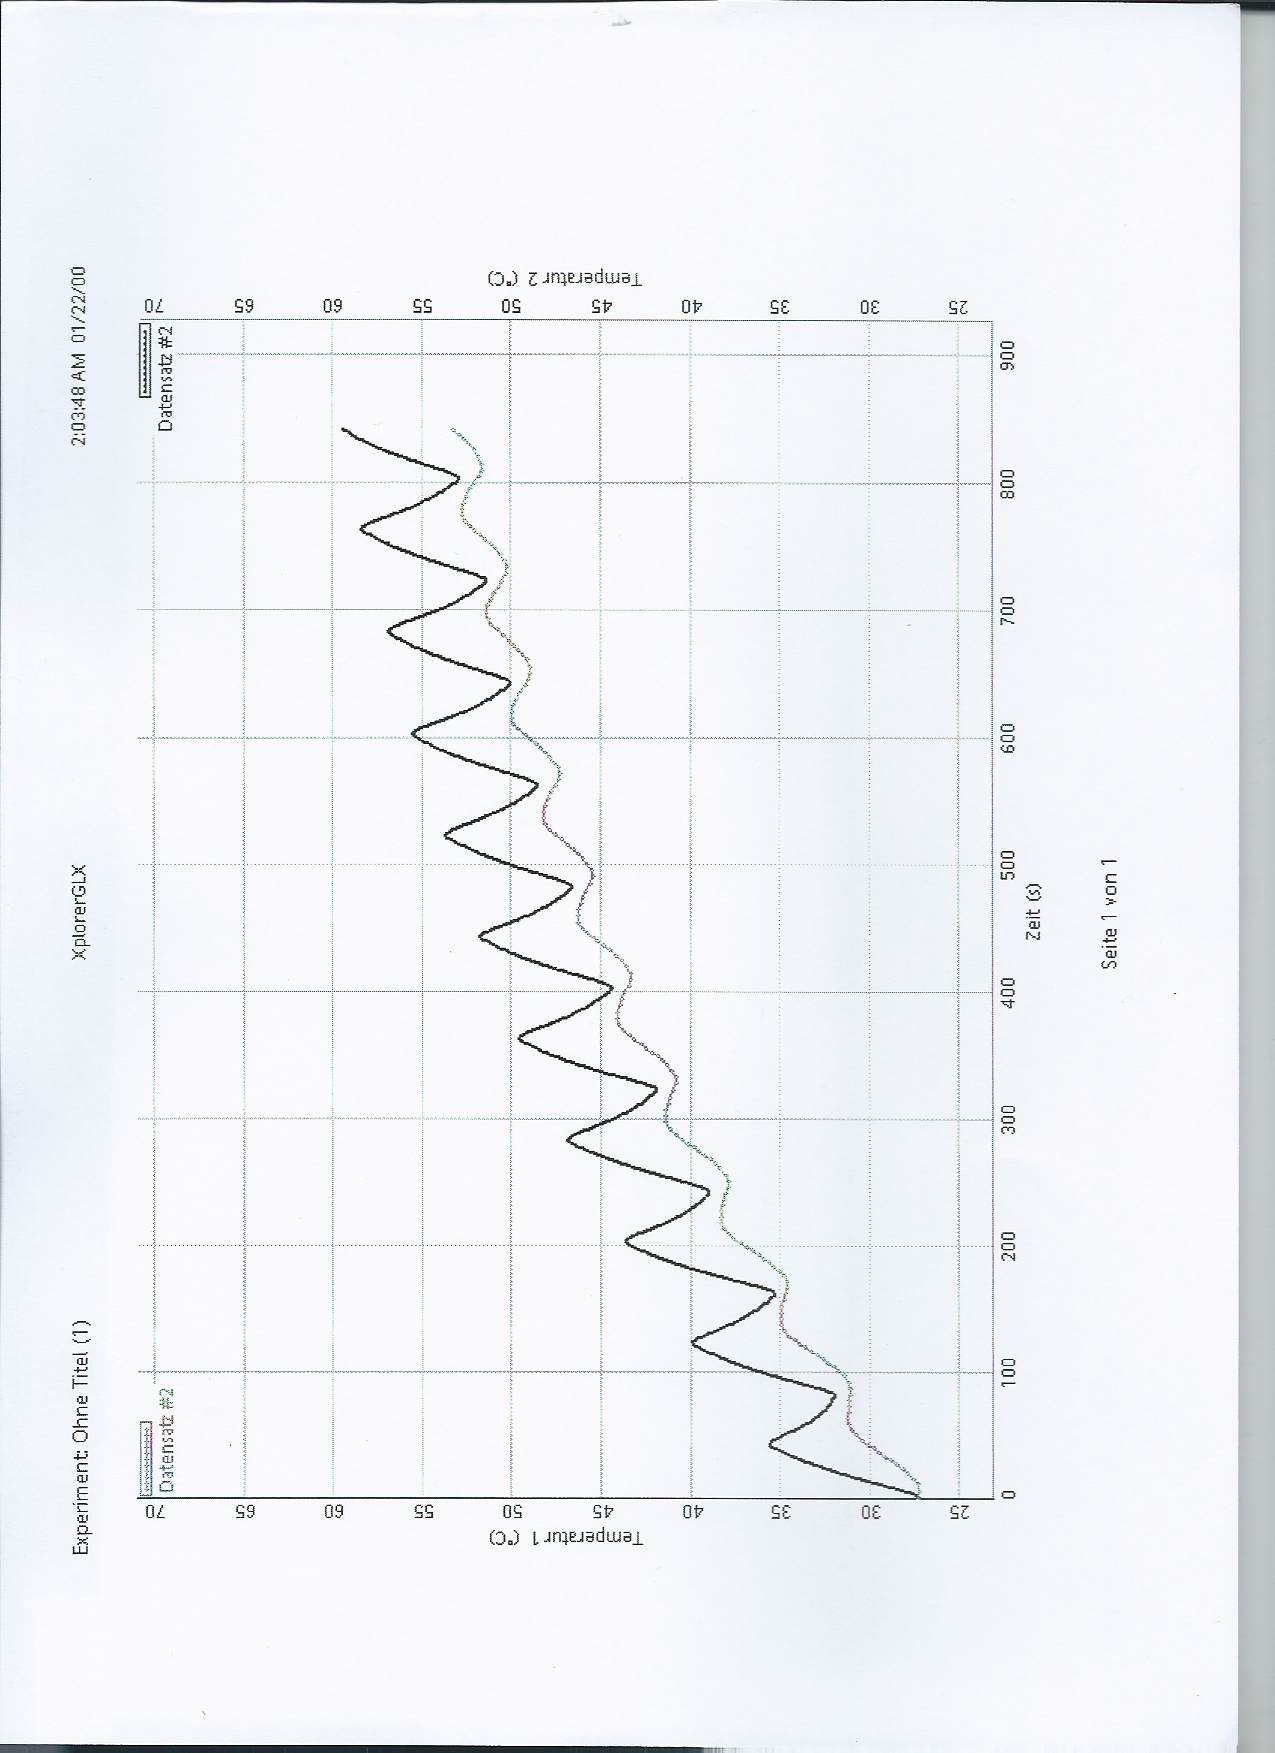
\includegraphics[height=13cm, angle=270]{scan-3.jpg}
  \caption{Zeitlicher Verlauf der Temperaturen für $T_1$ und $T_2$ bei periodischer Erwärmung nach der Angström-Methode.}
  \label{fig:5}
\end{figure}

Aus diesem Graphen können die Amplituden sowie zeitlichen Lagen der Maxima bestimmt werden.
Diese Werte sind in Tabelle \ref{tab:3} angegeben.

\begin{table}
  \centering
  \caption{Maxima der Temperaturen $T_1$ und $T_2$.}
  \label{tab:3}
  \sisetup{table-format=1.2}
  \begin{tabular}{c c c c}
    \toprule
    {$A_1 \:/\: \si{\kelvin}$} & {$A_2 \:/\: \si{\kelvin}$}  & {$t_1 \:/\: \si{\second}$}  & {$t_2 \:/\: \si{\second}$}\\
    \midrule
    \input{build/dyn1.tex}
    \bottomrule
  \end{tabular}
\end{table}


%\begin{table}
%  \centering
%  \caption{Beispieltabelle}
%  \label{tab:tabelle_beispiel}
%  \sisetup{table-format=1.2}
%  \begin{tabular}{c c}
%    \toprule
%    {$a [\si{\second}]$} & {$b [\si{\kelvin}]$}\\
%    \midrule
%    1.0000  & 11.00 \\
2.0000  & 12.00 \\
3.0000  & 13.00 \\
4.0000  & 14.00 \\
5.0000  & 15.00 \\
6.0000  & 16.00 \\
7.0000  & 17.00 \\
8.0000  & 18.00 \\
9.0000  & 19.00 \\
10.0000 & 20.00 \\

%    \bottomrule
%  \end{tabular}
%\end{table}
%
%Es ergibt sich
%\begin{align}
%  a &= (0 \pm 0) ~ \si{\joule\per\kelvin\per\gram}
 \\
%\end{align}
